\section{Abbildungs- und Tabellenverzeichnis erstellen}

In einer größeren, komplexen Arbeit, wie ein Fachbuch, hat man wahrscheinlich Tabellen und die eine oder andere Abbildung. Wenn man für diese eigene Verzeichnisse erstellen möchte, gibt es in Latex dafür passende Befehle. Diese Befehle sind \\listoffigures und \\listoftables. Damit die Befehle auch etwas zeigen, werden ein Bild und eine Tabelle gezeigt. Die beiden Befehle schreibt man in die Präambel.

\section{Abbildungen}

\subsection{Bitmap-Grafiken platzieren}

Abbildungen sind ein wesentlicher Bestandteil von Sach- und Fachbüchern, sowie von Sach- und Fachartikeln. Sie lockern lange Textpassagen auf und veranschaulichen Zusammenhänge.

Für dieses Beispiel wird eine Bitmap-Grafik eingebunden und verschieden platziert. Als erstes soll das Bild in Originalgröße zentriert eingebunden werden.

\begin{figure}[H]
	\centering
	\includegraphics[width=0.95\textwidth]{./images/ThaiBananen}
	\caption{Unreife Bananen aus Thailand -- Originalgröße}
	\label{fig:thai-bananen}
	\end{figure}
	
Mit der Angabe der Breite gibt man an, wieviel Prozent des Papiers das Bild in Anspruch nehmen soll, abzüglich der Seitenränder. 1.0 entspricht hierbei 100 \%, also die gesamte Breite. In diesem Beispiel wurde eine Breite von 0.95 gewählt, damit das Bild an beiden Rändern ein wenig eingerückt wird.

Im nächsten Beispiel soll das Bild auf der linken Seite eingebunden werden. Hierzu muss man das die figure-Umgebung entsprechend anpassen.


\begin{figure}[H]
		\includegraphics[width=0.4\linewidth]{./images/ThaiBananen-skaliert}		
		\caption{Thai-Bananen verkleinert und linksbündig}
		\label{fig:thai-bananen-skaliert-links}
\end{figure}
		
Wenn man Grafiken rechtsbündig platzieren möchte, muss der Bereich links vom Bild ausgefüllt werden. Dies erreicht man mit dem Befehl \textit{hfill} (steht für horizontal fill).
		
\begin{figure}[H] % [H] forces the figure to stay here
	\hfill % fill the horizontal space until it reaches the image
	\includegraphics[width=0.4\textwidth]{./images/ThaiBananen-skaliert} % tell LaTeX how much space the image should take up
	\caption{Thai-Bananen verkleinert und rechtsbündig}
	\label{fig:thai-bananen-skaliert-rechts}
\end{figure}


\subsection{Diagramme und Vektorgrafiken platzieren}

In diesem Abschnitt geht es um Diagramme und Vektorgrafiken, denn was ist eine gute Facharbeit ohne Diagramme? Um es simpel zu halten, kann man ein Diagramm, das man mit einer speziellen Software erstellt hat, z.B. Mermaid, in ein PDF umwandeln, da LaTeX von Haus aus keine SVGs unterstützt. Das PDF kann dann wie eine Bitmap-Grafik eingebunden werden, indem man das graphicx-Paket verwendet:

\begin{figure}[H]
	\centering
	\includegraphics[width=0.95\textwidth]{./images/OAUTH2-PKCE-Flow}
	\caption{OAUTH2-PKCE-Flow-Diagramm}
	\label{fig:oauth2-pkce-flog-diagramm}
\end{figure}

Nun, das sieht nicht richtig aus. Das Diagramm nimmt eine ganze Seite in Anspruch, obwohl es deutlich kleiner ist und es ist auch nicht zentriert. Was ist passiert?

Beim Export eines Diagramms kann es vorkommen, dass man nicht aufpasst und die Standard-Einstellungen verwendet. In dem Fall wird das Diagramm auf eine DIN-A4-Seite platziert, auch wenn es kleiner ist. LaTeX bindet nun das PDF so ein, wie es ist, mit allem Freiraum. Das heißt, das PDF selbst ist zentriert, das Diagramm ist jedoch immer noch in der linken oberen Ecke des PDFs. Daher ist das Diagramm nicht zentriert.

Bei Drawio kann man beim Export die Option \textit{Zuschneiden} wählen, was dann nur das Diagramm als PDF exportiert, ohne eine ganze Seite zu beanspruchen.

Das überarbeitete Diagramm sieht nun folgendermaßen aus:

\begin{figure}[H]
	\centering
	\includegraphics[width=0.95\textwidth]{./images/OAUTH2-PKCE-Flow-beschnitten}
	\caption{OAUTH2-PKCE-Flow-Diagramm-beschnitten}
	\label{fig:oauth2-pkce-flog-diagramm-beschnitten}
\end{figure}

Das Ergebnis sieht deutlich besser aus. Das Diagramm nimmt keine ganze Seite mehr ein und ist korrekt zentriert.

\newpage

\subsection{Grafiken in LaTeX erstellen mit TikZ}

Um Grafiken direkt in LaTeX zu erstellen, benötigt man spezielle Pakete, nämlich TikZ oder PSTricks, wobei TikZ das weiter verbreitete sein dürfte. Hat man das volle LaTeX-Paket installiert, sollte TikZ bereits enthalten sein, so dass kein extra Schritt notwendig ist.

Wie gewohnt bindet man das Paket in der Präambel mit \textit{usepackage} ein. Ein einfaches Dreieck kann man wie folgt zeichnen:


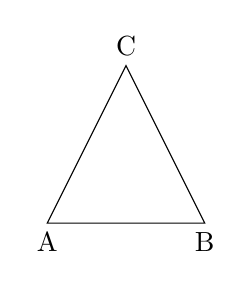
\begin{tikzpicture}
	\draw (0,0) -- (2,0) -- (1,2) -- cycle;
	\node at (0,0) [below]{A};
	\node at (2,0) [below]{B};
	\node at (1,2) [above]{C};
\end{tikzpicture}

Das ist super, aber ein bisschen zu simpel. Wie wäre es, das Dreieck in die Mitte zu schieben, zu vergrößern und Farbe zu geben?

\begin{center}
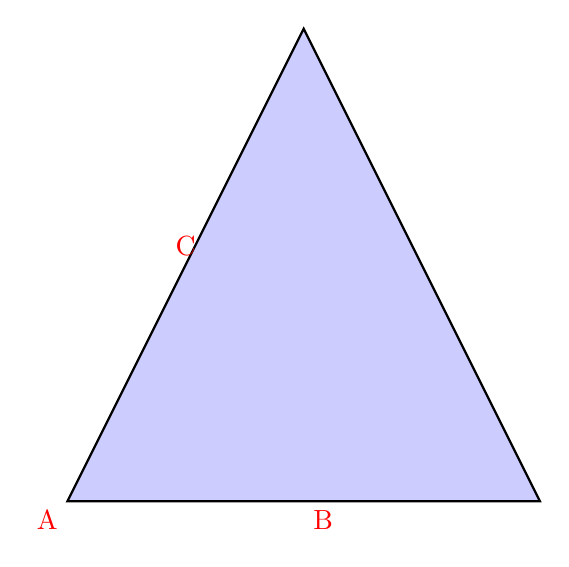
\begin{tikzpicture}[scale=1.5]
	\coordinate (A) at (0,0);
	\coordinate (B) at (4,0);
	\coordinate (C) at (2,4);
	
	\draw[fill=blue!20, draw=black, thick] (A) -- (B) -- (C) -- cycle;
	
	\node at (0,0) [below left, text=red]{A};
	\node at (2,0) [below right, text=red]{B};
	\node at (1,2) [above, text=red]{C};
\end{tikzpicture}
\end{center}

Das sieht schon besser aus, ist aber noch nicht rund -- die Labels sind nicht so platziert, dass es ein stimmiges Bild gibt. Hier sind also noch einige Anpassungen nötig.

\begin{center}
	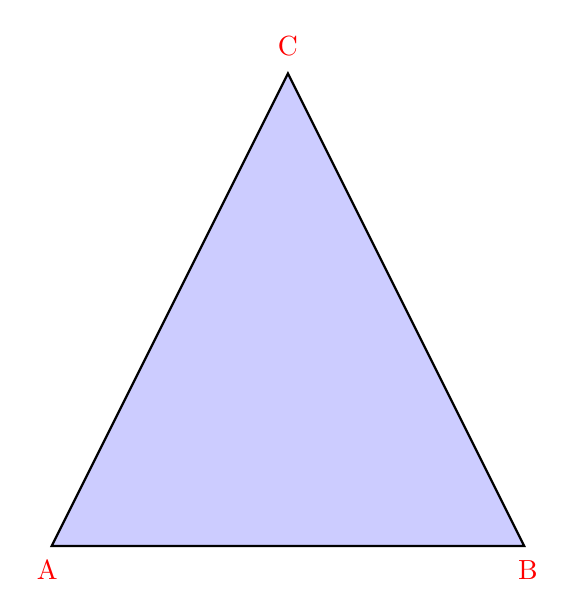
\begin{tikzpicture}[scale=1.5]
		\coordinate (A) at (0,0);
		\coordinate (B) at (4,0);
		\coordinate (C) at (2,4);
		
		\draw[fill=blue!20, draw=black, thick] (A) -- (B) -- (C) -- cycle;
		
		% correct the positions of the labels
		% position left node
		\node[anchor=east, xshift=2mm, yshift=-3mm, text=red] at (A) {A};
		
		% position the right node
		\node[anchor=west, xshift=-2mm, yshift=-3mm, text=red] at (B) {B};
		
		% position the node on the tip
		\node[anchor=south, yshift=1mm, text=red] at (C) {C};
	\end{tikzpicture}
\end{center}

Betrachtet man die Ergebnisse und welcher Aufwand nötig ist, sieht man schon, dass man bei komplexeren Diagrammen und Grafiken schnell ein recht komplizierten und umfangreichen Quelltext bekommt. Wer experimentieren möchte, kann noch 3D-Effekte hinzufügen oder dem Dreieck einen Schatten geben. Das ist aber eindeutig über dem hinaus, was der Artikel zeigen kann.